\chapter{Background}

By the mid 1960's  the popularity of online time-sharing computers created new concerns about security. It was shown that an employee could easily undermine all of the systems safeguards. By the end of the decade computer penetration became a major issue and the United States Department of Defence issued a major report on the subject. The DoD turned to Willis Ware (American Computer Pioneer) to form a task force comprised of experts from NSA, CIA, DoD, academia, and industry to assess the security risks of Computer penetration \cite{infosec2018}. From this report, government and business began to put together teams that would try to find vulnerabilities in computer networks and systems to protect the computer systems from unethical hacking or penetration. So-called tiger teams\footnote{Today, Penetration Testing teams have been renamed, from tiger teams, to red teams.}, named after specialized military teams, were formed in the late 1960s to test the ability of computer networks to resist an attack.

One of the early pioneers in penetration testing development and perhaps the leading computer penetration expert during these formative years was James P. Anderson. He worked with the NSA, RAND, and other government agencies to study system security. In his 1972 report, Anderson outlined a series of definitive steps that tiger teams could take to test systems for their ability to be penetrated and compromised. Anderson's approach included first identifying vulnerability and designing an attack on it, and then finding the weakness in the attack itself and ways to neutralize its threat. This fundamental method is still in use today.

James P. Anderson continued his research on securing computer systems during the 1970s and 1980s, with many of his publications and methods forming part of today's standard system protection.

Today, on-demand penetration testing is one of the latest methods to test a network system for ways it could be breached and information accessed. This hybrid approach to testing a network combines the manual and real-time attempts by ethical hackers to breach a system's security alongside automated tools that run checks on the system on a regular basis. 

\section{Understanding Penetration Testing}

Penetration Testing or PenTesting is a test performed on a computer network by a penetration tester or auditor for security purposes. A group of many testers is called tiger team/red team \cite{whitaker2006}. Penetration testing can be defined as a legal and authorized attempt to locate and successfully exploit computer systems for the purpose of enhancing the system's security. The process includes probing for vulnerabilities as well as providing proof of concept (POC) attacks to demonstrate the vulnerabilities are real. Such a test, involves simulating real attacks in real-time environments, encompassing a wide range of activities and variations, to assess the risk associated with potential security breaches \cite{shrestha2012}.

\section{Objectives of Penetration Testing}

\subsection{Origin of Vulnerabilities}
Penetration Testing is used to determine and detect vulnerabilities in a system. Such vulnerabilities may originate from improper system configuration, outdated components (software or hardware), lack of hardware and many other sources. The most impactful and eventually the most harmful one is human error. One of the most intriguing findings from IBM's "2014 Cyber Security Intelligence Index" is that 95 percent of all security incidents involve human error \cite{ibm2014}. It is the most common root for jeopardy since misuse of tools, unsafe transmittal of data to other, third-party or unknown entities, are some of the mistakes a person can make, willfully or not. More specifically, according to Verizon's "2013 Data Breach Investigations Report", 95 percent of those advanced and targeted on human error attacks, involved spear-phishing scams with emails containing malicious attachments that can cause malware to be downloaded onto the user's computing device \cite{verizon2013}. This gives attackers a foothold into the organization from which they can move laterally in search of valuable information, such as intellectual property.

\subsection{Penetration Testing's Purpose}
Penetration Testing involves acting as an actual attacker and performing the steps that one would take. From discovering the potential flaws of the organization's IT infrastructure, to abusing and carrying out an attack against those flaws in order to define the risk and impact of a possible exploitation. The intent of this procedure is to spot those weaknesses, narrow down security risk and prevent an attack by regulating the system's vulnerabilities and strengthening its security. Some of the most fundamental reasons to adopt and perform Penetration Tests are \cite{aicpa2018}\cite{saindane2015}:

\begin{itemize}

\item\textbf{Defining Security Posture}
\\ Even the most well managed and robust network infrastructures can be exposed to cyberattacks. Executive Management can determine to what extent an organization's vulnerabilities can potentially be exploited by hackers and the level of security their methods of protecting data provide.

\item\textbf{Improving Security of Organizations' Infrastructure}
\\Penetration testing is performed with the objective of improving the security of computer systems such as firewalls, routers and servers. Different security mechanisms like Intrusion Detection System(IDS), firewall, and cryptography are used to protect data. However, the frequency and severity of network intrusion, data theft and attacks caused by malicious code, hackers, disgruntled employees continue to increase along with the risks and costs associated with network security breaches and data theft. Penetration testing helps to address such concerns.

\item\textbf{Risk Mitigation}
\\ A well-executed penetration test provides a detailed overview of an organization's exploitable vulnerabilities and includes actionable recommendations on how a security engineer can optimize your protection levels in the short-term, mid-term and long-term. Discovered vulnerabilities are listed in order of 
\begin{enumerate}
\item how easily they can be exploited and
\item their impact on the organization in case of exploitation.
\end{enumerate}  

By following a so-called "risk-oriented prioritization" approach, information security executives will be able to prioritize these risks based on their criticality, plan their remediation efforts and allocate their security resources accordingly. For example, they may want to prioritize fixing the most critical vulnerabilities with the biggest negative impact on the organization first, and delay working on vulnerabilities that have light impact and are harder to exploit. This process will decrease risk of a possible event and its potential resulting impacts.

\item\textbf{Avoiding Data Breach}
\\A data breach is a security incident in which sensitive, protected or confidential data is copied, transmitted, viewed, stolen or used by an unauthorized entity. It is important for an organization to maintain the three security principles:
\begin{enumerate}
\item \textbf{The \textit{confidentiality} of the information.} Informational confidentiality is what comes to mind most frequently when we consider cybersecurity breaches-if an attacker is able to access private information and use it for nefarious purposes, confidentiality has been broken.
\item \textbf{The \textit{integrity} of the information.} Informational integrity refers to information in its original format that hasn't been manipulated by a bad actor.
\item \textbf{The \textit{availability} of the information.} Informational availability can be impacted by DDOS attacks. If an attacker is able to bring down a service for a period of time, it affects whether people can access the information they want or need.
\end{enumerate} 
To avoid such attacks, PenTesting assists in securing computer systems and important data, and eventually in eliminating unintentional information disclosure. 

\item\textbf{Reducing Financial Losses}
\\ Verizon's 2018 Data Breach Investigation Report shows that "76 percent of breaches were financially motivated" \cite{verizon2018}. Once security risks are considered and mitigated, cost benefits include reducing risk and exposure to internal and external threats and positioning the company to avoid potential financial loss from misuse of data, loss of data or noncompliance to policy, regulations or standards.Expenses on retrieving lost data and on recovering after a cyberattack might be tremendous since company's reputation will also be harmed.

\item\textbf{Enhance Organization's Reputation}
\\ Reputation benefits may include protecting the organization's brand and prestige, positioning the company as a trusted business partner and improving public opinion as if it considerately protects intellectual property and potential clients' sensitive data.

\end{itemize}

\section{Penetration Testing Types}

To uncover the vulnerabilities and security flaws, there are three types of Pen Testing which can be used. The type of penetration testing normally depends on the scope and the organizational wants and requirements. Following are the types of PenTesting \cite{whitaker2006}\cite{pci2015}:
\begin{itemize}
\item Black Box Test
\item White Box Test
\item Grey Box Test
\end{itemize}


\begin{figure}[ht!]
\centering
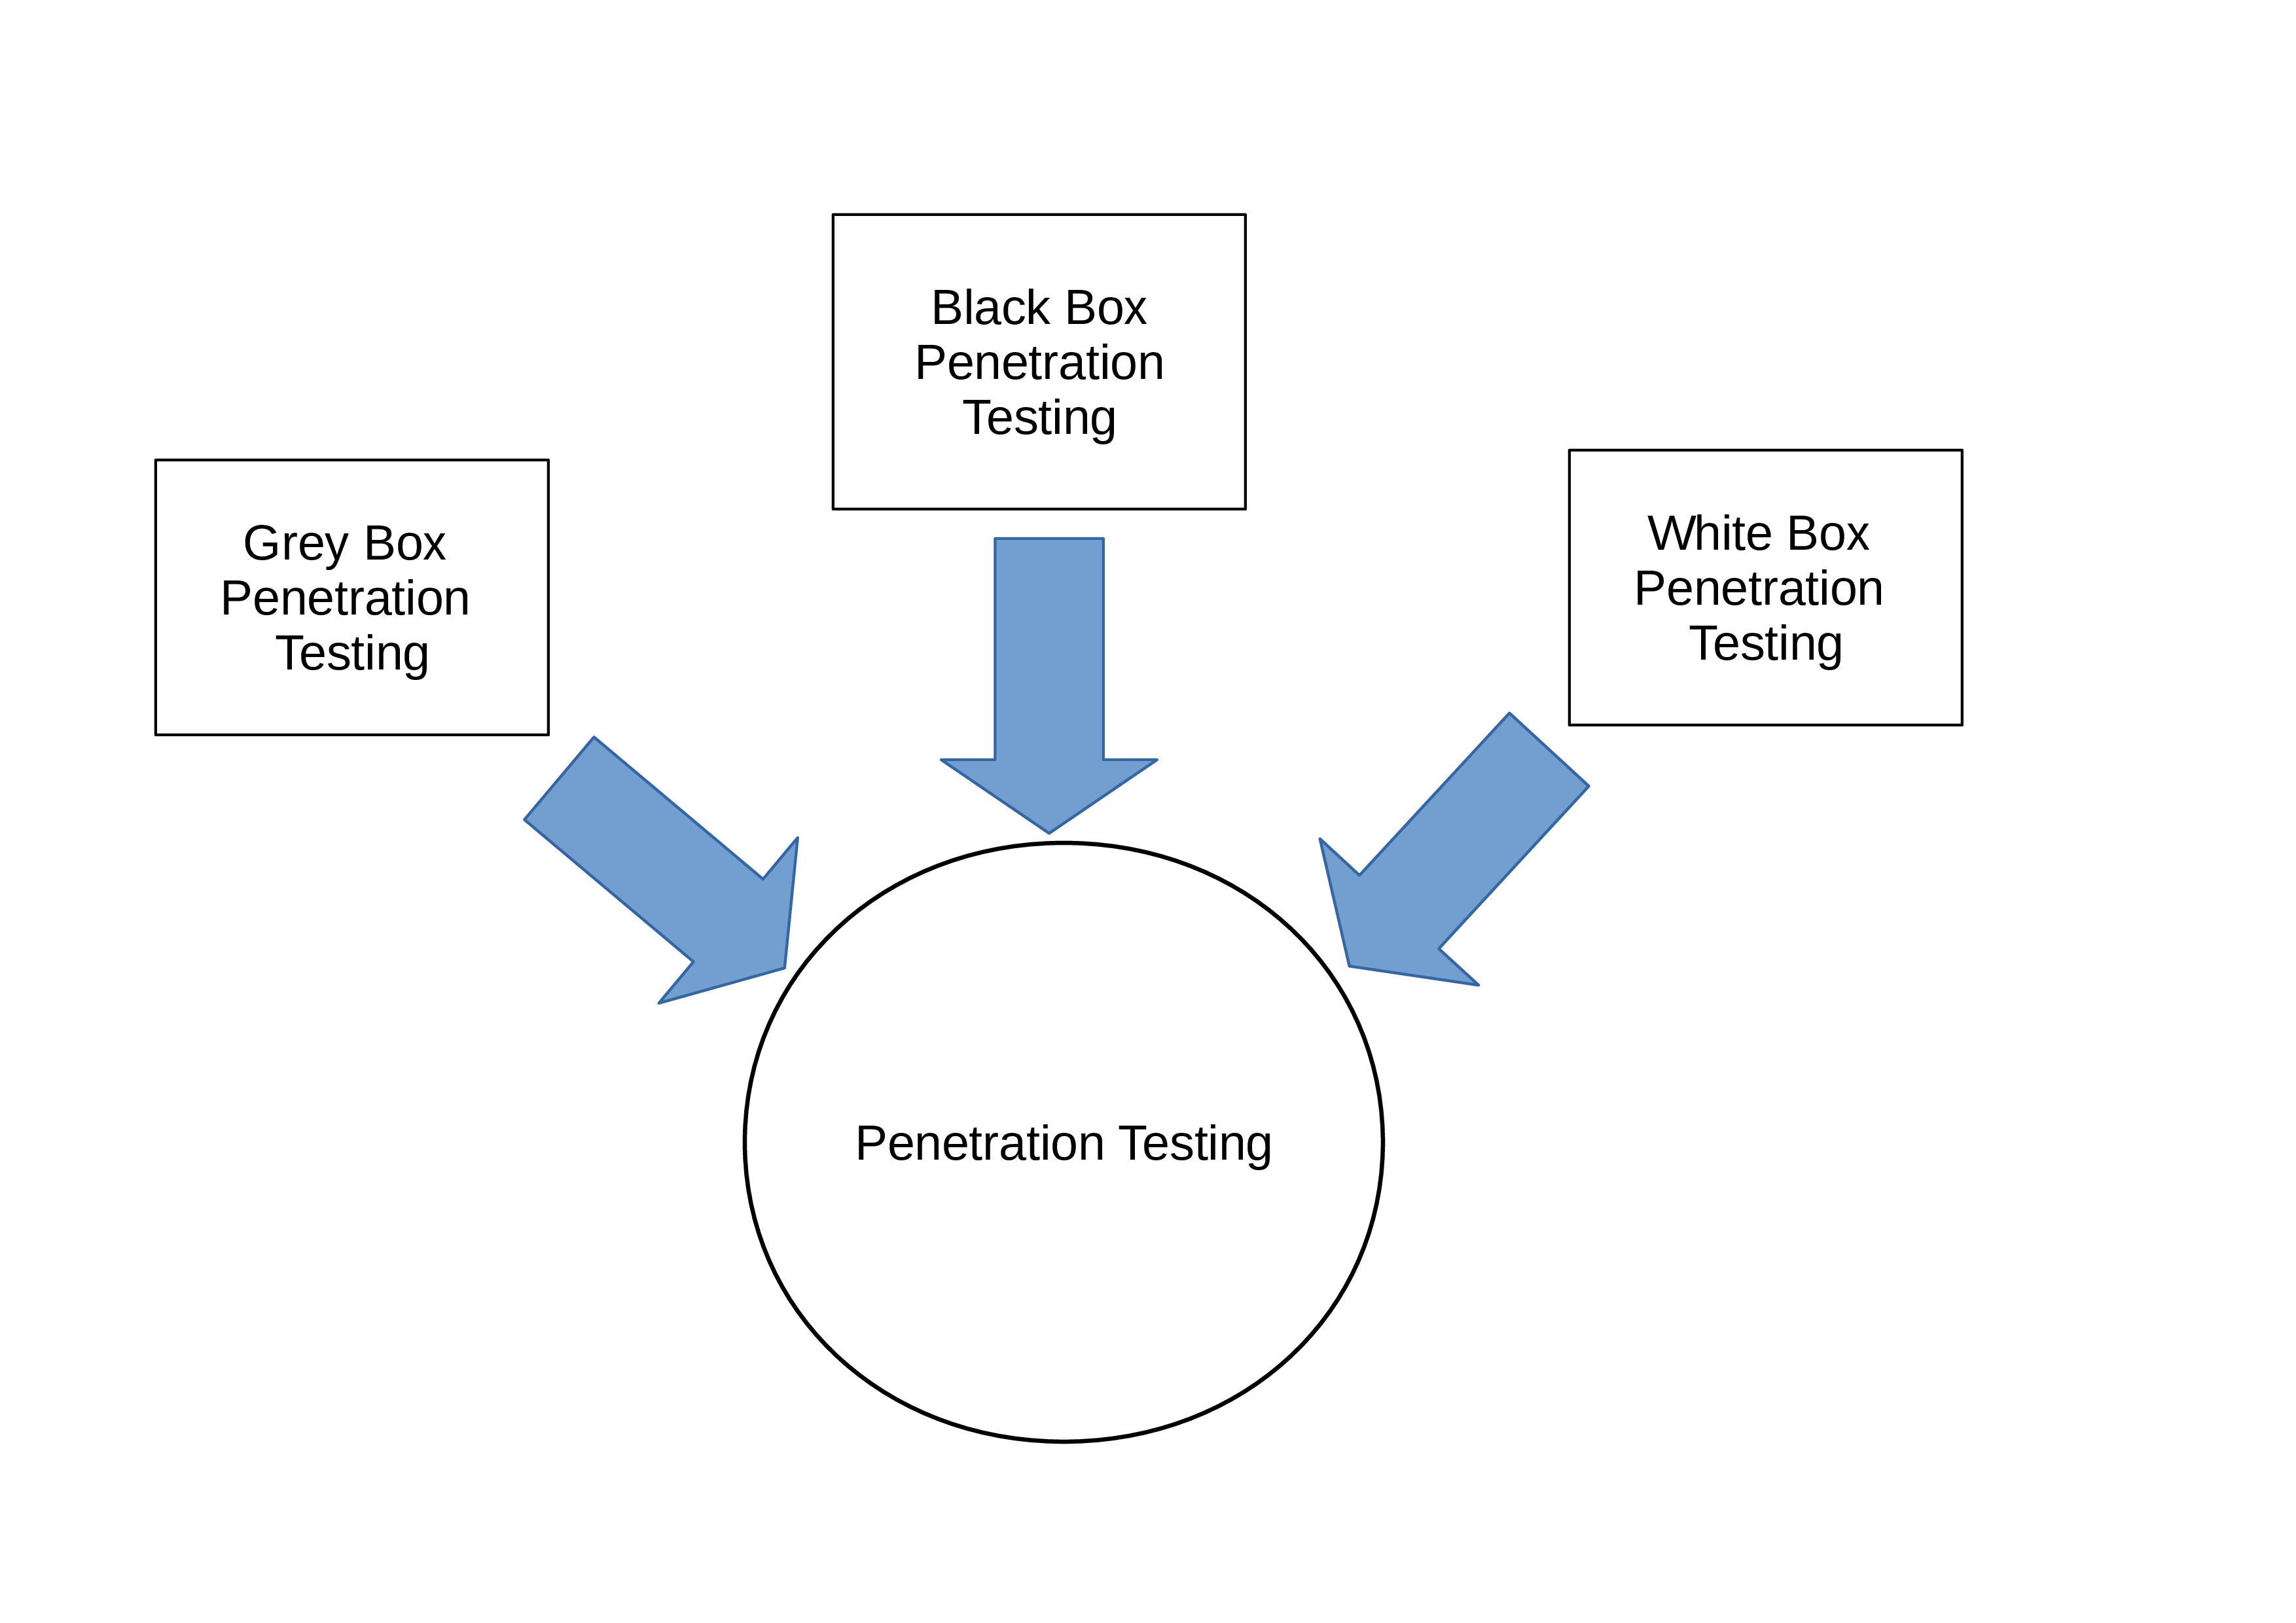
\includegraphics[width=0.9\textwidth]{Resources/General/PenTestingTypes.jpg}
\caption{Types of Penetration Testing \label{types}}
\end{figure}

\subsection{Black Box Test}
The penetration tester has no prior knowledge of a company network. There is no information given to the tester about the internal workings and the architecture of the system. As a result, this particular type of test can take a very long time to complete, so very often, the tester will rely upon the use of automated processes to completely uncover the weaknesses and vulnerabilities. This type of test is also referred to as the "trial and error" approach. For example, if it is an external black-box test, the tester might be given a website address or IP address and told to attempt to crack the website as if he were an outside malicious hacker.

The biggest advantage of this type of Penetration Testing, is that the attacker simulates the environment and the conditions of an actual attack since the test is generally conducted with the perspective of a user, not the designer.

Two major disadvantages are, firstly, this kind of test cases are difficult to design and secondly and most important, it does not cover every aspect of the security of the network and doesn't uncover every weakness.

\subsection{White Box Test}

In this type of Pentest, also known as "Clear Box Testing," the tester has complete knowledge of the internal network. The tester might be given network diagrams or a list of operating systems and applications prior to performing tests. Advantages of White Box Testing are:
\begin{itemize}
\item A White Box Test can be accomplished in a much quicker time frame when compared to a Black Box Test. 
\item Although it is not the most representative of outside attacks, it is the most accurate because it presents a worst-case scenario where the attacker has complete knowledge of the network and can be more explicit.
\item It finds the design errors that may have occurred because of the difference between logical flow of the program and the actual execution.
\end{itemize}

But, this approach also has its set of disadvantages. First, since a tester has complete knowledge, it could take more time to decide on what to focus specifically on regarding system and component testing and analysis. Secondly, to conduct this type of test, more sophisticated tools are required such as that of software code analyzers and debuggers.


\subsection{Grey Box Test}

With the Gray Box Test, both manual and automated testing processes can be utilized. A tester is usually provided partial or limited information about the internal details of the system. It can be considered as an attack by an external hacker who had gained illegitimate access to an organization's network infrastructure documents. It carries the following advantages:

\begin{itemize}
\item The tester does not require the access of source code, it is non-intrusive and unbiased.
\item No need to provide internal information about the system functions and other operation.
\item  With this particular method, there is a higher probability that more hard to find "security holes" will also be discovered as well.
\end{itemize}

\section{Vulnerability Assessment and Penetration Test}
A common misconception in the field of Computer Security, is that Penetration Testing and Vulnerability Assessment are the same functions and are used to accomplish the same goals. Unfortunately, in many cases, these two terms are incorrectly used interchangeably. This section aims to clarify differences between those two and demonstrate that both are integral components of a well-rounded vulnerability management program \cite{doshi2015}. 


\begin{description}
\item[Vulnerability Assessment] is a proactive and systematic strategy to discover vulnerabilities. The motive for vulnerability assessments is to yield lists of weaknesses, often prioritized by severity and/or business criticality.

Vulnerability assessment is achieved using scanners. It is a hybrid solution, which combines automated testing with expert analysis. It is a two step process whereas searching for vulnerabilities and reporting are the actions that consist that kind of assessments. 

\begin{figure}[ht!]
\centering
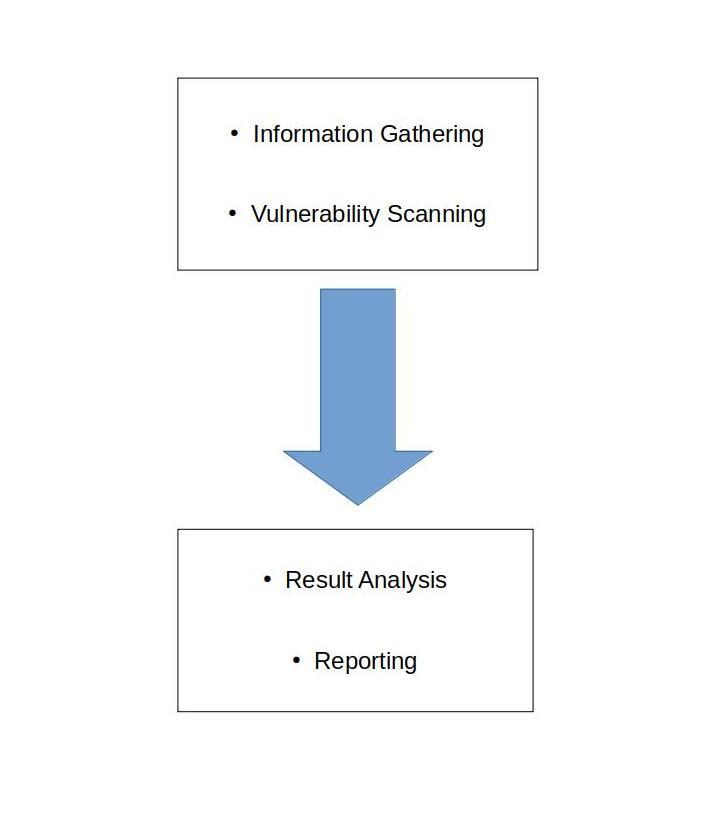
\includegraphics[width=0.7\textwidth]{Resources/Tools/VulnAssessment.jpg}
\caption{Procedure of a Vulnerability Assessment \label{VulAssessment}}
\end{figure}


\item[Penetration Testing] as described earlier, evaluates the security of a computer system or network by simulating an attack.
\end{description}


Concluding, on a Pentest, as opposed to a Vulnerability Assessment, takes a step beyond considering the testers not only discover exposures that could be used by attackers but also exploit the identified vulnerabilities, where possible, to assess what attackers might gain after a successful exploitation.

\begin{figure}[ht!]
\centering
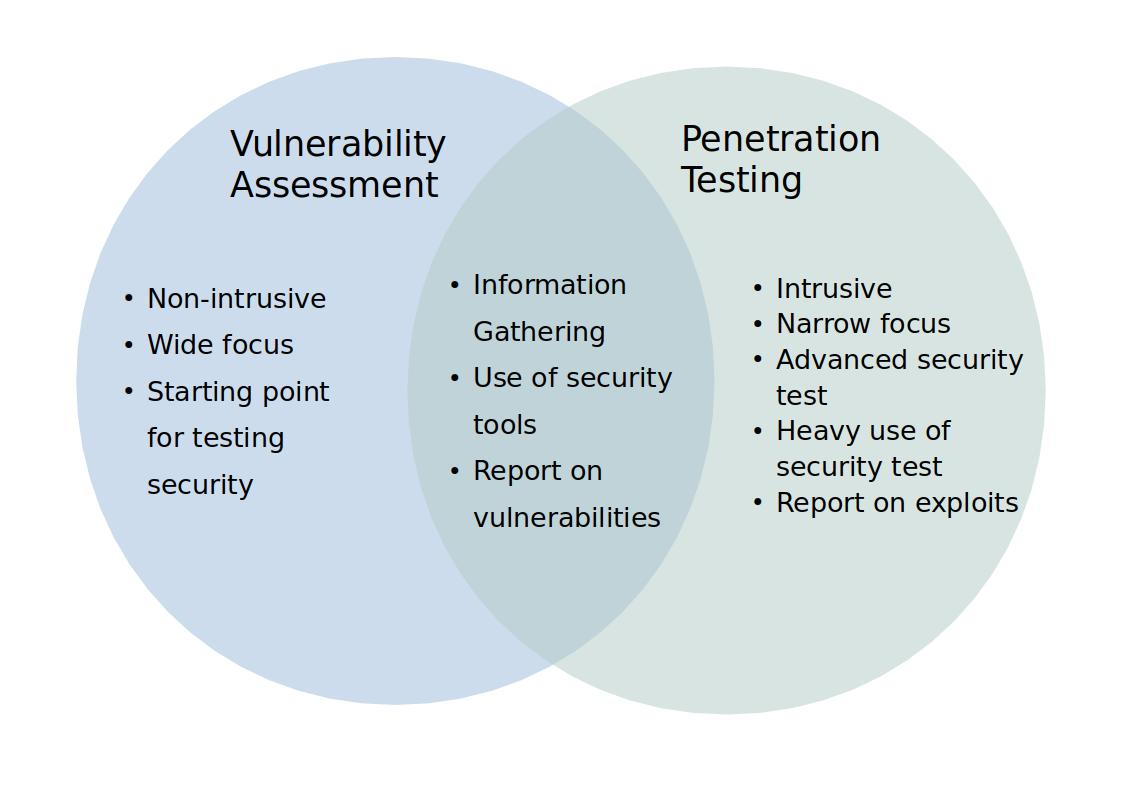
\includegraphics[width=0.9\textwidth]{Resources//General/PenTVulnAsComparison.jpg}
\caption{Common Fields and Comparison \label{Comparison}}
\end{figure}

\section{Manual and Automated Penetration Test}
\emph{Manual Penetration Testing} is a very detailed and complex process that requires a complete team of advanced and experienced security professionals, possessing diverse skill-sets, in order to be performed. Testers typically write their own exploits and choose the appropriate tools to master and use. Also, they need to be in control of the all the tasks and be present during the process of testing. Considering those factors, in short-term, manual testing seems to be low-efficient financially and time-wise. On the other hand, it has more benefits on the long term efficiency because of its universality and its ability to adapt in to changes made in the system or setbacks tester's might face.

\emph{Automated Penetration Testing} is considered a simple and cost efficient way of performing all tasks related to penetration testing. A commercial-base automated penetration testing solution is typically developed by a team of security professionals. An organization may also hire a firm or a group of professionals to produce a customized automated test depending on the system's architecture and design or the organization's requirements. In such a test most of the tasks are automated, so it can be less time-consuming than manual penetration testing. The ease of reproducibility of the tests is also a big benefit. Figure \ref{Manual versus Automated} shows a comparison of those two tests focused on the automation's benefits \cite{stefinko2016}.

\newpage
\begin{figure}[H]
\centering
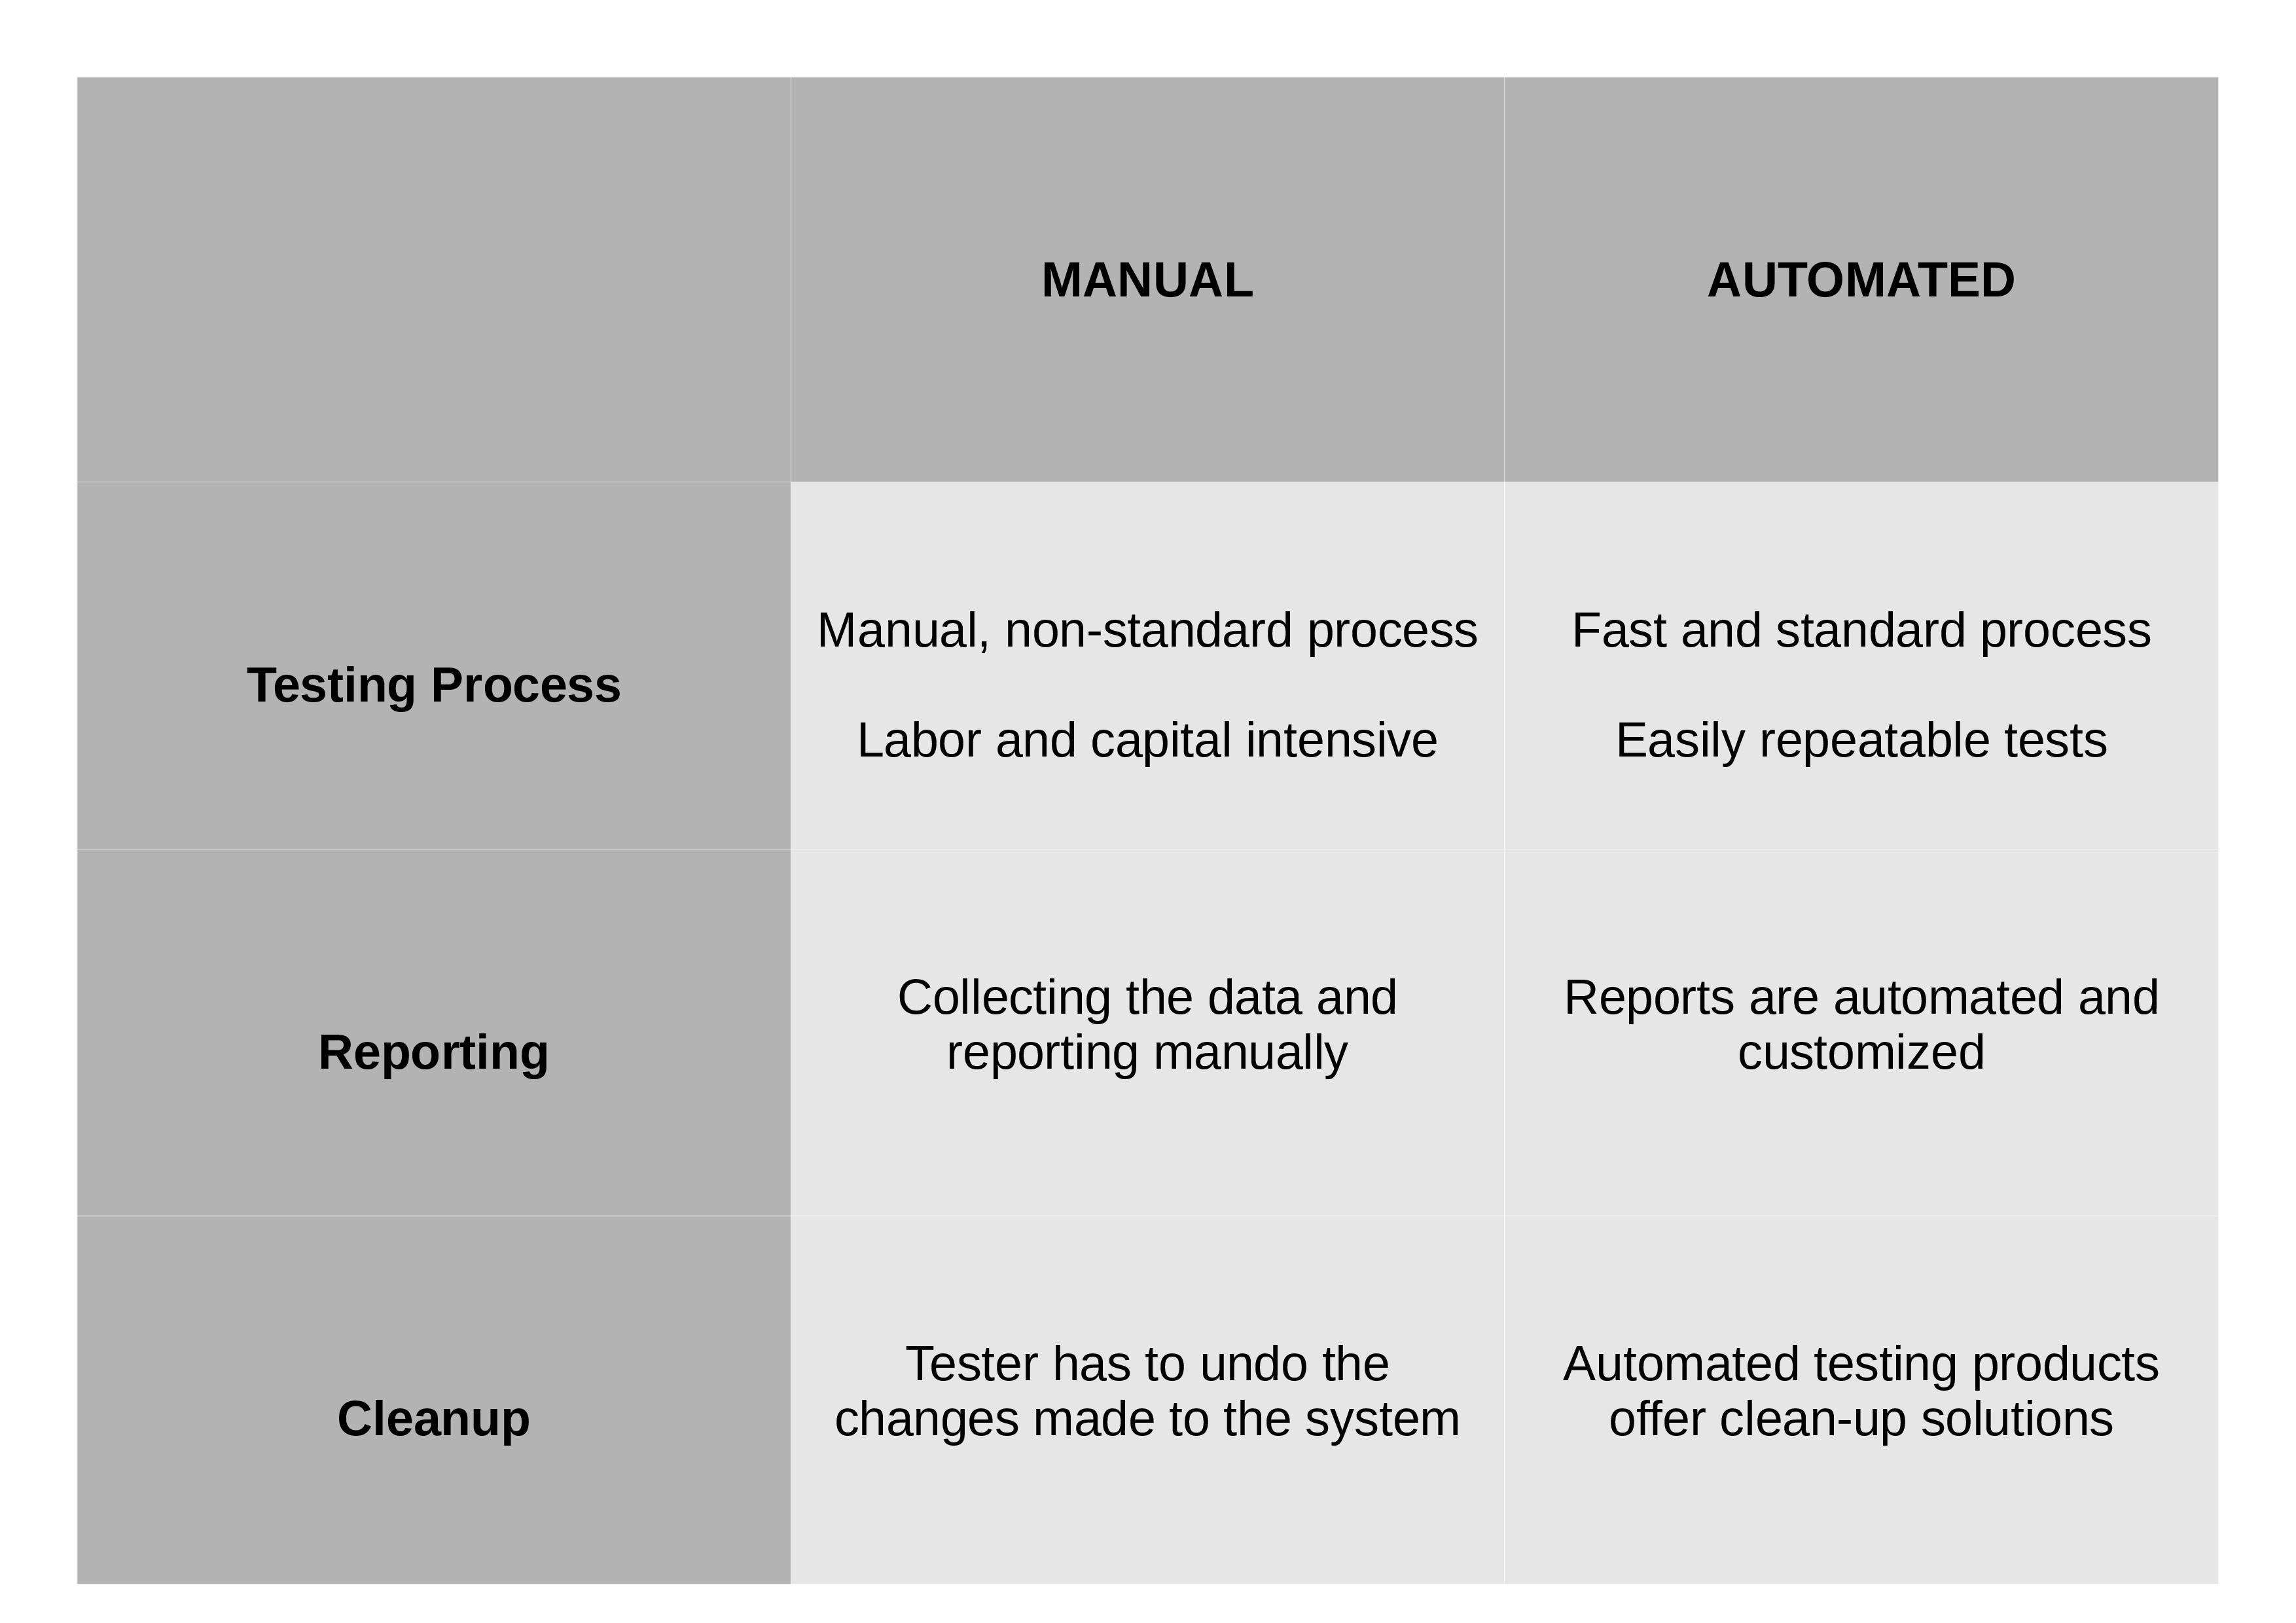
\includegraphics[width=1.0\textwidth]{Resources/General/ManvsAuto.jpg}
\caption{Manual versus Automated Testing \label{Manual versus Automated}}
\end{figure}

A conclusion on this subject might differ from choosing one or the other type of test, since both have their own unique benefits. As the Department of Computer Science of North Carolina State University concludes in their case study, a combination of both might be the most beneficial choice since each type of test might discover different types of vulnerabilities, offering a better overall security posture in the end \cite{austin2011}.



\section{Rules of Engagement}
Rules of Engagement refer to how each aspect of the test will be conducted. To ensure effectiveness and efficiency of a test, the red team must determine the parameters that define and characterize the Penetration Test to correspond to the requirements and rules set by the organization. Prior to the act of testing, the organization and the testing team agree upon the conditions in which testing is to be performed and the degree of exploitation, if any, that is permitted \cite{pci2015}\cite{nist2008}.

\subsection{Scope Definition}
Defining scope is arguably one of the most important components of a penetration test. The scope of a project specifically defines what is to be tested. Scoping a test is the first step one should take in order to perform a test. The breadth of the test is mostly defined by the organization on which infrastructure the test is being performed and the testers. Commonly, the organizations set the parameters of the procedure, depending on their needs. On the other hand, in case it is up to the red team to decide, testers should consider many factors and features for the test such as the extent of the system to be tested, the prior information base of the test or the technique \cite{nist2008}.

\subsection{Approach}
The focus of a test may vary depending on the system infrastructure. Many tests consist of more than one techniques. Using many different approaches can lead to better understanding of the security of the system and providing more information on it. Some techniques are \cite{ptes2011}:

\begin{itemize}
\item Network Oriented
\item Web Application Focus
\item Wireless Network Testing
\item Physical Penetration Test
\item Social Engineering
\end{itemize}

\subsection{Starting Point and Information}
As described above, a test may be categorized depending on the knowledge the tester has about the computer system, prior to testing. According to the information a PenTester is provided, the test can then be characterized as a Black, Grey or White Box Test \cite{ptes2011}.

\begin{itemize}
\item In a \textbf{white box test}, testers have or are provided with a complete knowledge regarding the target network or system infrastructure. This testing can be considered as a simulation of an attack by any who might be in possession of the system knowledge.
\item In a \textbf{black box test}, testers aren't provided with information regarding the target system architecture. This testing can be considered as a simulation of a real-world attack by an outsider.
\end{itemize}

\subsection{Reach}
Determining which parts of the system are to be tested is an important step to set the rest of the scope. The organization might choose a limited or focused part of the system to examine, and not the overall security of the infrastructure, in order to spot weaknesses on a specific part. Adopting a more focused range of attack offers reduction of the complexity and cost of the test. The time spent for a penetration testing is also directly linked to the scope of the systems to be investigated \cite{ptes2011}. 

\subsection{Aggression}
Tests may be performed with different degree of aggressiveness. Ranging from passive/cautious to aggressive which is the most noticeable attack, the tester must decide to what intensity the vulnerabilities may be exploited since system disruptions might occur. Some example of such aggressive attacks is buffer overflows used on target systems and Denial of Service (DoS) attacks. Such attempts will cause weakening or malfunction of the system, so this factor must be taken into consideration \cite{ptes2011}.


\section{Legal and Ethical Considerations}
A broad term is used when referring to laws and regulations on computer systems and the Internet, called Cyberlaw/IT law. It is one of the newest areas of the legal system because internet technology develops at such a rapid pace. Understanding cyberlaw is of the utmost importance. Cyberlaw does not constitute a separate area of law rather it encompasses aspects of contract, intellectual property, privacy and data protection laws. Intellectual property is an important component and falls into the following categories \cite{whitaker2006}\cite{harris2007}:

\begin{enumerate}
\item Copyright
\item Patents
\item Trademarks/Service Marks
\item Domain Disputes
\item Contracts
\item Privacy
\item Employment
\item Data Retention
\end{enumerate}

Laws differ from country to country but security professionals should be familiar with these laws, since they are expected to work in the construct the laws provide. Also,  any attempt or act of hacking outside workspace is illegal and immoral. Even though penetration testers might have significant knowledge on cybersecurity, using them without permission and outside of their workspace is not permitted.


Ethical responsibilities are also significantly important in the process of penetration testing. Any client of a penetration testing firm must be convinced that the testers will not attempt any unauthorized access, data theft or any types of attack that isn't allowed by the testing contract, in order for the client to trust the firm and its testers. A tester must not speak or share any of the actions performed or vulnerabilities discovered during the process of penetration testing, considering that these types of information are critical for the security and brand name of the infrastructure. Responsibilities do not stop when the test is done, however. After the test is completed, Confidentiality of the test results must be ensured and in no case those results should be shared to or obtained by a third-party \cite{harris2007}. 



\section{Security Testing Standards and Methodologies}

There are some Open-Source and public methodologies that have been widely accepted and practice among the penetration test. They are used to assist and guide the tester during the process of designing and performing a test. One may be counselled by a Penetration Testing Standard and adjust it in order to fit the test's requirements. Most common among other frameworks are:

\begin{itemize}
\item Information Systems Security Assessment Framework (ISSAF)
\item National Institute of Standards and Technology (NIST 800-115)
\item Open Source Security Testing Methodology Manual (OSSTMM)
\item Open Web Application Security Project Testing Guide (OWASP Testing Guide v4)
\item PCI Penetration Testing Guide (PCI)
\item Penetration Testing Execution Standard (PTES)
\end{itemize}

\subsection{National Institute of Science and Technology}
The National Institute of Science and Technology (NIST) of the U.S. government produced Special Publication 800-115 \textit{Guideline on Network Security Testing} in order to expand and improve upon their previous guide, NIST Special Publication 800-42, \textit{Guideline on Network Security Testing}, which it replaced. This standard addresses and covers network penetration testing methodologies at a high level. The technical guidance presented in this document is as follows \cite{nist2008}:

\begin{itemize}
\item Developing a security testing policy
\item Roles and Responsibilities of assessment
\item Testing Techniques
\item Incident Response
\item Data Handling
\item Risk Analysis
\item Report
\item Post-Test Actions
\end{itemize}

\subsection{Open Source Security Testing Methodology Manual}
\textit{Open Source Security Testing Methodology Manual} (OSSTMM) is a peer-reviewed manual of security testing, analysis and metrics which result in verified facts. These facts provide actionable information that can measurably improve operational security. The overall document is very extensive, covering various kinds of security tests. Although it does not get into depth with specific commands and tools, but is still profoundly valuable. Topics tackled in the OSSTMM include the competitive \textbf{intelligence review} (conducting reconnaissance against the target enterprise), Internet \textbf{security analysis} (finding and acquiring open ports and vulnerabilities in Internet accessible systems), and \textbf{communications security} (addressing vulnerabilities commonly found in PBXs, modems, and fax machines). It also provides a thorough guide for a presentation of metrics on a professional level and correlation of test results in a consistent way. Because of the metrics and the statistical view this document provides, the OSSTMM methodology reduces the occurrence of false positives and false negatives and provides accurate measurement for the security \cite{osstmm2010}.

\subsection{Open Web Application Security Project}
Nowadays, more and more applications become Internet based, so the need to examine the Web application security rises. This is where \textit{OWASP Testing Guide} stands on. This guide is an open-source project that provides a testing framework for http-based applications. It focused on covering the area of web applications and services in depth instead of having a wider and more general scope, targeting more than one area of cyber security.

The breadth of this framework spreads from \textbf{Session Management Testing, Input Validation Testing} and \textbf{Client Side Testing} to \textbf{Configuration}, \textbf{Deployment Management Testing} and \textbf{Business Logic Testing} \cite{owasp2014}.

\subsection{Payment Card Industry Data Security Standard}

The \textit{Payment Card Industry Data Security Standard} (PCI DSS) Penetration Testing guideline provides a very good reference of the penetration testing area while it's not a hands-on technical guideline to introduce testing tools. This guidance focuses on the following \cite{pci2015}.

\begin{itemize}
\item \textbf{Penetration Testing Components.} Comprehension of the diverse segments that make up a properly designed penetration test and how this contrasts from a vulnerability scan.
\item \textbf{Qualifications of a Penetration Tester.} Deciding the capabilities of a tester.
\item \textbf{Penetration Testing Methodologies.} Accurate data associated with the three primary parts of a penetration test: 
\begin{enumerate}
\item pre-engagement
\item engagement
\item post-engagement
\end{enumerate}
\item \textbf{Penetration Testing Reporting Guidelines.} Assistance for building up a comprehensive penetration test that incorporates all the necessary content and properly defining risk.
\end{itemize}

\subsection{Penetration Testing Execution Standard}
\textit{Penetration Testing Execution Standard} (PTES) covers a wide spectrum of the process, from the initial communication and reasoning behind a PenTest, through the intelligence gathering and threat modeling phases where testers are working behind the scenes in order to get a better understanding of the tested organization, through vulnerability research, exploitation and post exploitation, where the technical security expertise of the testers come to play and combine with the business understanding of the engagement, and finally to the reporting, which captures the entire process, in a manner that makes sense to the customer and provides the most value to it \cite{ptes2011}.
PTES defines penetration testing as 7 phases:
\begin{enumerate}
\item Pre-engagement Interactions
\item Intelligence Gathering
\item Threat Modeling
\item Vulnerability Analysis
\item Exploitation
\item Post Exploitation
\item Reporting
\end{enumerate}

\section{Composition of a Test}
As every process, penetration testing can be broken down in to a series of rules and steps. Those steps set the methodology for performing a test. This methodology gives a practical source of documentation for formalizing any uniquely designed penetration test plan. It is the plan that the tester is going to follow. There are different penetration testing methodologies that one can choose from and there is no such thing as "the right methodology". The selection of the proper methodology must be precise, careful and fit the requirements of the penetration test as much as possible \cite{nist2008}. 

Before deciding on the methodology, as mentioned before, setting the scope and the rules of engagement is crucial. This first step will be the breaking point in order to correctly decide on the proper penetration testing methodology that satisfies the requirements the most and adjust it according to the scope that was decided on.

\begin{description}
\item[Planning] is the starting point of a penetration test. It is the initiation of a test since the rules are being determined and the testing goals are set . It is the foundation for a successful penetration test.
\item[Discovery] consists of two parts. First part is the beginning of the actual testing and covers  the act of gathering preliminary data or intelligence on the target. The data is gathered in order to better plan for your attack. This part can be performed actively (meaning that you are directly touching the target) or passively (meaning that your recon is being performed through an intermediary). Such examples are network host name and IP address information or employee names  and contact information. The second part of the discovery phase requires the application of technical tools to gather further intelligence on your target, but in this case, the intel being sought is more commonly about the systems that they have in place. A good example would be the use of a vulnerability scanner on a target network. In a more broad term, this part of discovery may also be called as "Vulnerability Analysis".
\item[Attack] Third phase, attacking, requires taking control of one or more devices by exploiting previously identified potential vulnerabilities  in order to either extract data from the target, or to use that device to then launch attacks on other targets. Penetration testers must consider that taking the steps involved in being able to be persistently within the target environment in order to gather as much data as possible, is crucial and stealth during this stage is important.
\item[Reporting] is the last phase of the activity. This phase can occur in parallel to the other three phases or at the end of the Attack. The final report must be prepared keeping in mind both management as well as technical aspects, detailing all the findings with proper graphs, figures, etc. so as to convey a proper presentation of the vulnerabilities and it's impact to the business of the target organization.
\end{description}

Often, a tester will not have the maximum level of potential access to a system and, as a result, he might discover more vulnerabilities than the ones on which the test was planned upon, or any change in the state of the targeted system. If this occurs while performing an attack, additional analysis and examination of the system are required. Thus, the phase of discovery and attack are mutually connected in order to breakdown the additional data found and reevaluate the attacking plan the tester is going to follow.

\begin{figure}[H]
\centering
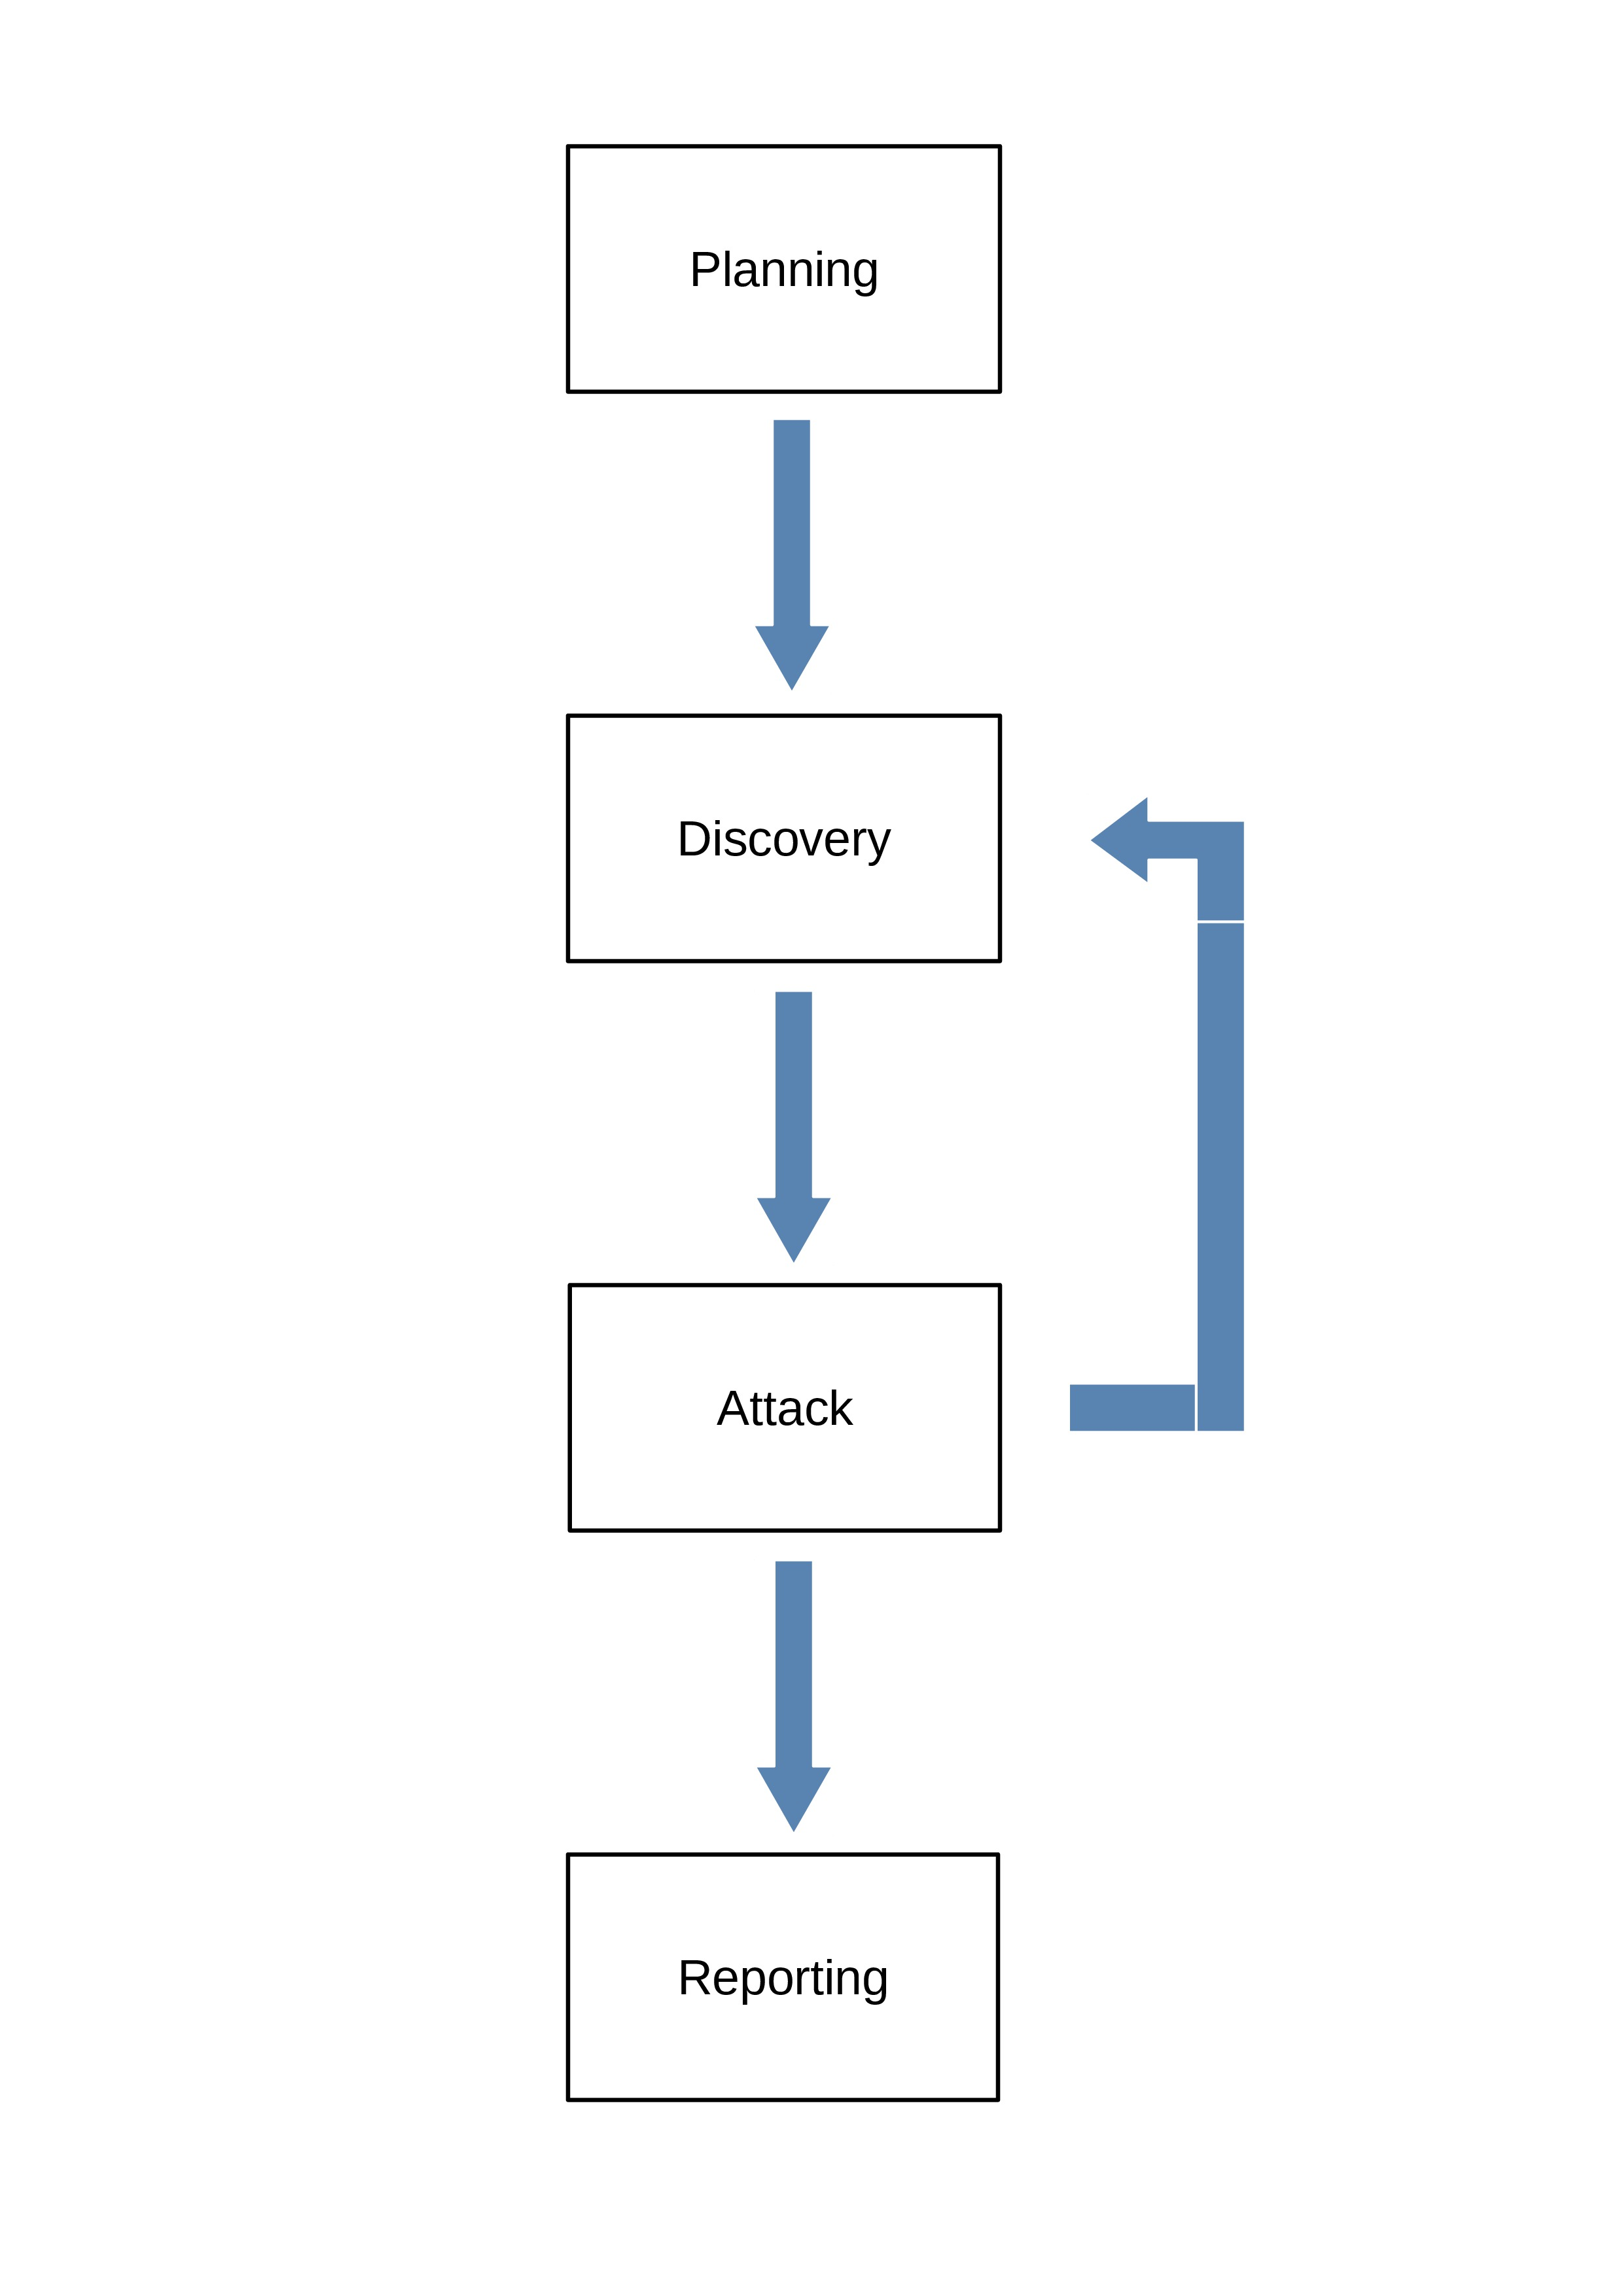
\includegraphics[width=0.7\textwidth]{Resources/General/PhasesGraph.jpg}
\caption{Penetration Testing Phases \label{Phases}}
\end{figure}

\subsubsection{Exploring the different tools}

After understanding the process of Penetration Testing and its steps, it is vital to familiarize with a more practical approach of the test by getting to know the tools used in a penetration testing environment and perform such attacks. As this thesis continues, a description of the different attack points to a targeted computer system and the associated tools, will be presented. 
